\section*{A 1.1}

\subsection*{a)}
The contents of the file \textit{assignment1.le} are shown below.

First the \texttt{reverse} function.
\begin{verbatim}
\ Assignment 1
(load listfunctions)

\ A function 'reverse' that reverses a list
(define reverse (lambda ((a . d)) (append (reverse d) (list a)) (a) a))
\end{verbatim}
The function is recursively appending its first element to the back of the list that is generated by using the reverse function on the tail of the list.

To implement the second function, \texttt{sort}, I have implemented a number of helper functions, as seen below.
\begin{verbatim}
\ Helper function: append two lists (even if both lists are ())
(define append2
   (lambda (() bs) bs
           (bs ()) bs
           (() ()) ()
           ((a . as) bs) (cons a (append2 as bs))
           (bs (a . as)) (append (list bs a) as)
           (as bs) (list as bs)))

\ Helper function: Find all elements smaller than p
(define allSmallerThan (lambda ((a . d) p) (append2 (< a p) (allSmallerThan d p))
                               (() p) ()
                               (a p) (< a p)))

\ Helper function: Find all elements greater than p
(define allGreaterThan (lambda ((a . d) p) (append2 (> a p) (allGreaterThan d p))
                               (() p) ()
                               (a p) (> a p)))

\ A function 'sort' that sorts a list
(define sort (lambda ((a . d)) (append (append (sort (allSmallerThan d a)) 
                                       (list a)) (sort (allGreaterThan d a)))
                     (()) ()
                     a a))

\end{verbatim}
The idea behind the code is to choose a pivot element, which is simply the first element of the given list, and then divide the rest of the list in to two different lists - one where all elements are smaller than the pivot element, and on where all elements are larger or equal. Now the sort function is used recursively on both lists. The function returns a list consisting of first the list with smaller elements (sorted), then the pivot element, and then the list with larger or equal elements (sorted).

\subsection*{b)}
Here are some examples of running \texttt{reverse}.
\begin{figure}[h]
    \centering
    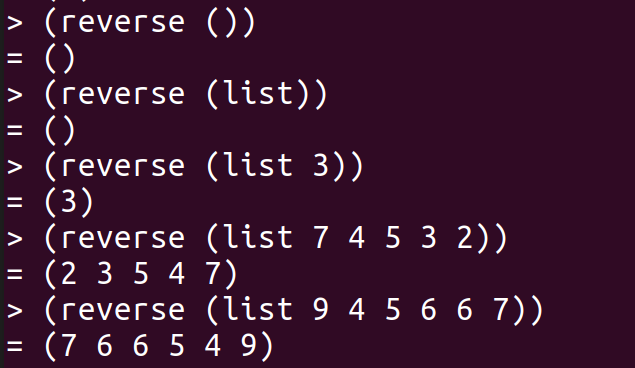
\includegraphics[width=0.5\textwidth]{rev.png}
    \caption{The reverse function}
\end{figure}

Here are some examples of running \texttt{sort}.
\begin{figure}[h]
    \centering
    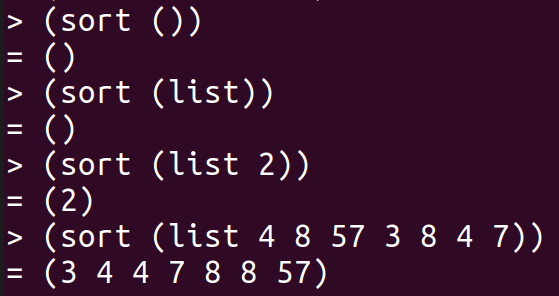
\includegraphics[width=0.5\textwidth]{sort.png}
    \caption{The sort function}
\end{figure}


\subsection*{c)}
I think the part of the syntax that was the most difficult for me to understand was the \textit{cons} operater, and the way the pattern matching work. I think the idea is pretty straight forward, but i spent quite a lot of time just trying out all of the operators to figure out exactly how they worked and what they returned.
